\section{Begrifflichkeiten}
In der Praxis sind viele, in dieser Arbeit häufig verwendete, Begriffe unterschiedlich belegt. Aus diesem Grund soll im Folgenden eindeutig klargestellt werden, was mit den verwendeten Begriffen tatsächlich gemeint ist.

\begin{description}
	\item [App (plural: Apps)]
		In dieser Arbeit werden Programme die speziell für Smartphones entwickelt wurden als Apps bezeichnet. Implizit wird hiermit auch die Plattform auf Android oder iOS eingrenzt. Der Begriff App zeichnet sich in dieser Arbeit dadurch aus, dass die damit gemeinte Anwendung für den Nutzer sehr einfach zu installieren ist. In der Regel beziehen Nutzer Apps aus einem Shop des Hersteller beispielsweise Apples AppStore und starten diese über ein Icon auf dem Startbildschirm des Betriebssystems.
		
	\item [Webseite, Webanwendung und Web App]
		Der Begriff Webseite wird in dieser Arbeit für HTML-basierte Inhalte verwendet, die der*die Nutzer*in über den Browser abruft.
		
		Die Webanwendung unterscheidet sich dahingehen, dass sie dynamisch auf den Nutzer reagiert und seine Eingaben auswertet und gegebenenfalls den angezeigten Inhalt ändert oder nachlädt. Speziell werden JavaScript basierte Anwendungen in dieser Arbeit als Webanwendung oder Web App bezeichnet. Web App und Webanwendung werden synonym verwendet.
		
		Eine Webseite kann, aber muss keine Webanwendung oder Web App sein.
	
	\item [Progressive Web App]
		Eine Progressive Web App ist eine Webseite und speziell eine Webanwendung oder Web App, welche dynamisch auf den Nutzer reagiert.
		In dieser Arbeit werden Webanwendungen, welche lokal auf einem Gerät installiert werden können als \acf{pwa} bezeichnet. Die PWA kann als Webanwendung oder Web App bezeichnet werden, welche die Kriterien aus Kapitel \ref{chap:pwa} erfüllt.
		
		Im Unterschied zur nativen App kann die selbe \ac{pwa} sowohl auf Smartphones, als auch auf eine Desktopgerät (Notebook, Desktop Computer etc.) installiert werden.
		
	\item [Desktop \ac{pwa}]
		Mit Desktop \ac{pwa} ist hier explizit eine Progressive Web App gemeint, welche auf einem Desktopgerät installiert wird.
			
	\item [native App]
		Diese Arbeit beschäftigt sich mit einer modernen Methode Mobilanwendungen zu programmieren: der \ac{pwa}. Im Unterschied dazu ist eine native App in Java oder Swift geschrieben und ist damit stark plattformabhängig. Nativ implementiere Apps sind entweder für iOS oder Android entwickelt worden, nicht aber für mehrere Plattformen.
		
	\item [Container]
		Da die Entwicklung von Apps stark am Frontend orientiert ist wird häufig der Begriff Container verwendet. Damit ist explizit \textit{kein Container im Sinne von Virtualisierung}, wie beispielsweise ein Docker-Container, gemeint. Der Begriff wird im HTML-Kontext verwendet und meint in dieser Arbeit ein Element, dass andere Elemente beinhaltet.
	
\end{description}

\section{Die Progressive Web App}
\label{chap:pwa}

%\subsection{Charakteristiken einer \ac{pwa}}
Zu Beginn dieses Unterkapitels soll die bereits erwähnte \acf{pwa} erklärt werden. Anschließend folgen die verwendeten Frameworks für die Entwicklung der \ac{pwa}. Ein Überblick über diese ist essenziell für das Verständnis von Kapitel \ref{chap:implementierung}, in welchem die Implementierungsschritte betrachtet werden.

Eine Progressive Web App ist ein nächster Schritt nach der Dynamisierung statischer HTML-Seiten durch JavaScript und Frontendframeworks. Der Software Entwickler und Autor Majid Hajian charakterisiert \ac{pwa}s mit acht Eigenschaften. Die wichtigsten dieser Charakteristika werden im Folgenden zusammenfassend erläutert:


\begin{description}
  \item [Installierbarkeit]
	  Der*die Nutzer*in einer Webanwendung kann diese lokal auf seinem Gerät installieren. Sie kann anschließend, wie eine native App, vom Startbildschirm gestartet werden. Um die Webanwendung zu Nutzen muss ein*e Nutzer*in keinen Zwischenschritt mehr über den Browser tätigen.
  
  \item [Ähnlichkeit mit einer nativ implementierten App]  
 	 Klassischerweise werden Android-Apps in Java und iOS Apps in Swift programmiert. Die \ac{pwa} soll, wie eine native App, auf die Hardware des Mobilgeräts zugreifen können (beispielsweise die Nutzung Bluetooth-Chips). Außerdem unterscheidet sich das User Interface der \ac{pwa} nicht maßgeblich von der nativen App. 
  
  \item [Offline-Verwendung] 
  	Die \ac{pwa} soll unabhängig von Netzwerkverbindung funktionieren. Sie ist nach dem "offline-first-design" konzipiert. Die Google-Chrome Dokumentation für Cloud-Entwickler beschreibt Offline First Apps als Webanwendung, deren Dateien (JavaScript, HTML, CSS etc.) bereits heruntergeladen sind. Daten werden temporär über eine Browser-Schnittstelle gespeichert und bei Bedarf synchronisiert. Außerdem kann die Anwendung auf eine unterbrochene Netzwerkverbindungen reagieren \cite{GoogleOfflineApps}. Die \ac{pwa} ist demnach eine Webanwendung, die sowohl online, als auch offline nutzbar ist.

  \item [Mobiloptimiert]  
  	Die \ac{pwa} ist für die (meist leistungsschwache) Mobilhardware konzipiert und funktioniert hierauf ohne Performanzprobleme. Hajian legt besonders auf das schnelle Laden beim Start der Anwendung wert.
  	
  \item [Informierung des*der Nutzers*in] 
  	Wie native Apps, kann die \ac{pwa} den Nutzer über Push-Nachrichten informieren oder zu Interaktion auffordern.
\end{description}

\cite[S. 1f.]{Hajian2019}
Diese Charakteristiken decken sich mit der Beschreibung durch die Entwickler-Dokumentation der \ac{pwa} von Google. Im Vergleich zu Hijian ist diese etwas spezifischer und erwähnt beispielsweise die Kontrolle des Anwendungscaches durch einen JavaScript Service Worker (siehe Kapitel \ref{chap:service_worker}), um die Abhängigkeit von einer Netzwerkverbindung aufzuheben.
\cite{GooglePWAOverview}

\subsection{Installation einer Progressive Web App}

Diese Arbeit betrachtet die \ac{pwa}, da sie (wie eine native Anwendung) lokal auf einem Gerät installiert werden kann. Es ist dafür kein zentraler Shop nötig: die Installation wird über den Browser gestartet.

\begin{figure}[h]
        \centering
        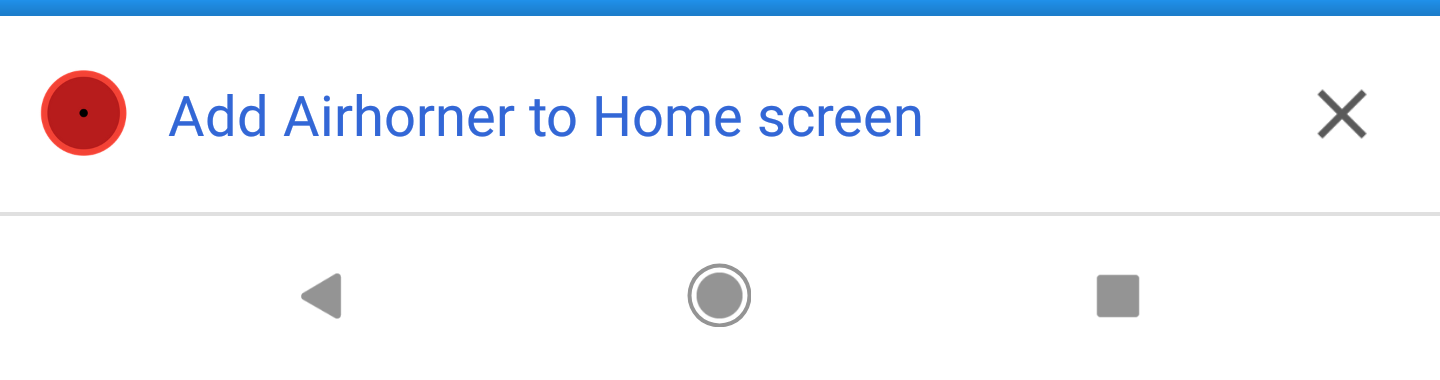
\includegraphics[scale=0.2]{img/a2hs-infobar-cropped.png}
        \caption{Browserdialog zur Installation einer \ac{pwa} \cite{PWAAddToHomeScreenPrompt}}
        \label{fig:pwainstallationprompt}
\end{figure}

Die Aufforderung zur Installation einer \ac{pwa} kann entweder über den Browser (siehe Abbildung \ref{fig:pwainstallationprompt}) erfolgen oder über ein Element der Website, dass ein Event erzeugt, wie beispielsweise ein Button oder ein Dialog. 

Zwar bezeichnen Browser die Installation meist nur als \texttt{Zum Startbildschirm hinzufügen} tatsächlich generiert der Browser aber dann eine WebAPK, welche auf dem Gerät installiert wird. Auf Desktopgeräte startet die \ac{pwa} in einem eignen stark verschlankten Browserfenster ohne Suchleiste und Bedienelemente. \cite{GooglePWAInstallation}


\subsection{Manifest Datei für die Konfiguration der \ac{pwa}}

Um die \ac{pwa} auf einem Gerät installieren zu können, muss es eine \textit{web-app-manifest} Datei zur Verfügung gestellt werden. Diese ist ein \ac{json} file, welche als Konfigurationsdatei der installierten Anwendung dient. \cite{GooglePWAManifest}

\begin{listing}[H]
    \inputminted{json}{sourcecode/manifest_sample.json}
    \caption{Manifestdatei einer \ac{pwa}}
      \label{sourcecode:manifest_sample}
\end{listing}

Quellcode-Abschnitt \ref{sourcecode:manifest_sample} zeigt den Inhalt einer Manifest-Datei. Neben diversen Icons (Zeile 4-15) werden auch \textit{Name} (Zeile 3), \textit{Farbschema} (Zeile 20) und \textit{Anzeigeeinstellungen} (Zeile 18) festgelegt.
Die Manifest-Datei wird im HTML der Webanwendung eingebunden, siehe Quellcode-Abschnitt \ref{sourcecode:manifest_include}. 

Es ist die Einfachheit dieses Prozesses hervorzuheben: Das Hinzufügen einer (wenige Zeilen langer) \ac{json}-Datei macht die gesamte Webanwendung installierbar. Es wird kein App-Store, manueller Dateidownload oder Installer benötigt. 

\begin{listing}[H]
    \inputminted{xml}{sourcecode/include_manifest.html}
    \caption{Einbinden der Manifestdatei}
      \label{sourcecode:manifest_include}
              %https://developers.google.com/web/fundamentals/web-app-manifest?hl=en
\end{listing}

%\begin{figure}[h]
%        \centering
%%        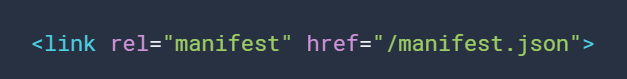
\includegraphics[scale=0.7]{img/include_manifest.png}
 %%       \caption{Einfache Einbindung des Manifests}
  %      \label{sourcecode:manifest_include}
        %https://developers.google.com/web/fundamentals/web-app-manifest?hl=en
%\end{figure}


\subsection{Service Worker für Offline-Funktionalität und Benachrichtigungen}
\label{chap:service_worker}

Damit die \ac{pwa} trotz fehlender Netzwerkverbindung funktioniert wird ein besonderer Mechanismus benötigt: der Service Worker. Mit ihm können Abhängigkeiten der App lokal gecached werden, so dass die Anwendung auch bei schlechter oder gar fehlender Netzwerkverbindung funktioniert. \cite[S. 7]{BeginningPWA}

Ein Service Worker ist ein von der UI separiert laufendes Hintergrundskript der Webanwendung, siehe Abbildung \ref{fig:serviceWorker}. Er wird genutzt um Bilder, Skripts, Styles oder ganze Seiten zu cachen. Bei bestehender Netzwerkverbindung führt er nötige Synchronisierungen durch. Nicht zuletzt ist er auch für das senden von Push-Notifications zuständig. \cite[S. 24]{BeginningPWA}

\begin{figure}[h]
        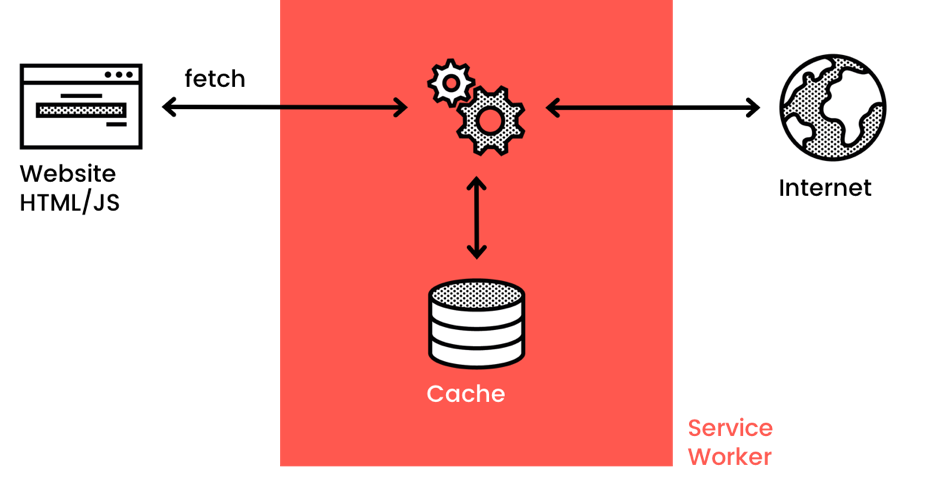
\includegraphics[width=\linewidth]{img/ServiceWorker-8a0968f1b295f1ff.png}
        \centering
        \caption{Konzept des Service Workers \cite{ServiceWorkerDiagramm}}
        \label{fig:serviceWorker}
\end{figure}


Alle verbreiteten Desktopbrowser wie Chrome, Firefox, Opera, Edge und mittlerweile auch Safari unterstützen das Service Worker Konzept. Der Mobile Chromebrowser unter Android unterstützt Service Worker bereits voll, während Safari unter iOS noch an diesem Feature arbeitet. \cite[S. 9]{BeginningPWA}


\subsection{Plattformen von eine \ac{pwa} aktuell unterstützen}
Das Projekt \textit{CanIUse} aggregiert Daten zu Webstandards des w3 Konsortiums und Browserdokumentationen. Es wird als Quelle für die Unterstützung von Features durch aktuelle Browser herangezogen.

Apples mobiler Browser Safari unterstützt eines der wichtigsten Features der \ac{pwa} noch nicht vollständig: das Web App Manifest. Allerdings wird der Service Worker vollständig unterstützt \cite{CanIUseWebManifest}. Wann und ob Safari die Unterstützung für das Manifest implementiert ist unklar und bleibt abzuwarten. Die aktuelle Teilunterstützung zeigt jedoch, dass sich Apple nicht grundsätzlich gegen die \ac{pwa} weigert.

 %Die Versionen zeigen aber eine stetig voranschreitende Integration der, erweitert den Funktionsumfang in den neusten Versionen von iOS. 

% https://medium.com/@firt/progressive-web-apps-on-ios-are-here-d00430dee3a7



% Source: https://developers.google.com/web/progressive-web-apps/desktop
Die Nutzung von \ac{pwa}s ist nicht ausschließlich auf Smartphones begrenzt. Wie normale Desktopprogramme werden Desktop \ac{pwa}s in einem eigenen Fenster gestartet. 
Der Unterschied zwischen den Bedienelementen nativer Desktopanwendungen und Desktop \ac{pwa}s ist ausschließlich farblicher Natur. Stark vereinfacht beschrieben, sind Desktop \ac{pwa}s Browserfenster ohne Tabs und Adressleiste. Durch die Nutzung von Service Workern, welche die Webanwendung cachen, sind auch Desktop \ac{pwa}s nicht an eine Netzwerkverbindung gebunden.

Grundsätzlich können Desktop \ac{pwa}s auf jedem Betriebssystem installiert werden, auf dem Google Chrome (Version größer 73) installiert werden kann: Windows, Mac, Linux und Chrome OS.
\cite{GooglePWADesktop}



\subsection{Grundlage der Webanwendung: JavaScript Laufzeitumgebung Node.js}

%NodeJSWebsiteAbout
\textit{Node.js} ist eine open-source JavaScript Laufzeitumgebung für die Entwicklung skalierbarer Webanwendungen 
\cite{NodeJSWebsiteAbout}.
Selbst baut Node.js auf der \textit{V8-Engine} auf, einer Laufzeitumgebung, die auch von Google Chrome genutzt wird 
%NodeJSRecepies
\cite[S. 1]{NodeJSRecepies}.
% PracitalNodeJS
Wegen zeitsparenden Features, wie automatischem Typecasting oder der Tatsache, dass Node.js alle Daten als Objekt behandelt, erfreut sich Node.js großer Beliebtheit 
\cite[S. 12]{PracitalNodeJS}.
Die Kombination mit dem \textit{Package Manager npm} ermöglicht die einfache Installation und Nutzung von Modulen, um die Funktionalität der Plattform zu erweitern. 
\cite[S. 9]{NodeJSRecepies}.


\subsection{Frontend-Framwork Angular für die Entwicklung von Webanwendungen}

Angular ist ein open-source TypeScript basiertes Framework zur Entwicklung von Webanwendungen, welches Node.js nutzt.


%https://octoverse.github.com/projects
Mit über Achttausend Mitwirkenden Entwicklern (Angular CLI) beziehungsweise über Siebentausend Mitwirkender (Angular Framework) belegt das Angular Command Line Interface und das Angular Framework die Plätze 4 und 6 der größten Projekte auf Github. 
% https://octoverse.github.com/projects
\cite{OctoverseGitHubStatistics}

Das Framework arbeitet auf Basis von Komponenten. Ein Eingabefeld, Seite oder eine Liste werden in Angular als solche Komponenten separat betrachtet. Auch in der Dateistruktur werden Komponenten stark getrennt. Jede Komponente besitzt beispielsweise ein eigenes CSS (oder SCSS) und HTML-File. Eine Komponente für eine Seite kann so auch eine oder sogar mehrere Listenkomponenten einbinden. Durch die Wiederverwendung von Code-Fragmenten in Komponenten wird der Programmcode sehr übersichtlich und strukturiert.

\begin{figure}[h]
        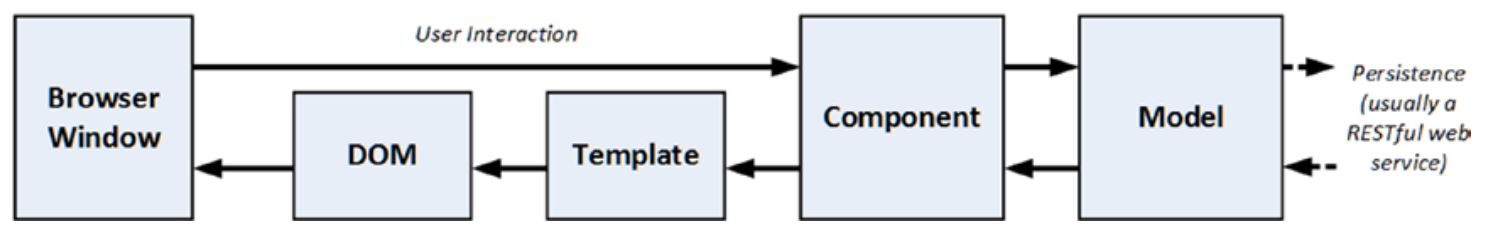
\includegraphics[width=\linewidth]{img/Angular_MVC.JPG}
        \centering
        \caption{MVC Konzept von Angular \cite[S. 35, Abbildung 3-4]{ProAngular}}
        \label{fig:angularmvc}
\end{figure}

Eine Angular Anwendung ist in drei Einheiten gegliedert:\\

\textbf{Model}\\ 
Enthält Logik für die Verwaltung von Daten, beispielsweise das Erstellen, Speichern oder Modifizieren. Dies kann über die Kommunikation mit einem Webserver via REST-API erfolgen. Das Model enthält keine Logik, um mit dem Nutzer zu interagieren.\\

\textbf{Component}\\
Enthält Logik für das Aktualisieren der Daten im Model aufgrund Nutzerinteraktion. \\

\textbf{Template}\\ 
Enthält Logik und Markup, um dem Nutzer Daten anzeigen zu können.

\cite{ProAngular}

\section{native Apps}


\subsection{Apple iOS} \label{chap:apple_ios}

iOS ist ein Betriebssystem, welches vom US-amerikanischen Technologiekonzern \textit{Apple, Inc.} im Rahmen des erstmalig vorgestellten \textit{iPhones} im Jahre 2007, damals noch unter dem Namen \textit{iPhone OS}, in Umlauf gebracht wurde. Stand heute läuft dieses Betriebssystem ausschließlich auf den Mobilgeräten des genannten Herstellers. Neben dem iPhone nutzt auch das Multimedia-Gerät \textit{iPod touch} das Betriebssystem iOS. Der Tabletcomputer \textit{iPad} wurde bis September 2019 ebenfalls über iOS betrieben, besitzt jedoch seit der Umstellung ein eigenes, an iOS stark angelehntes Betriebssystem \textit{iPadOS}.

\subsubsection{Entwicklung von iOS-Applikationen}

In seiner ersten Version stellte iPhone OS noch keinerlei Möglichkeit bereit, Anwendungen von Drittanbietern bereitzustellen sowie zu nutzen. Dies änderte sich bei der Umbenennung des Betriebssystems in iOS im Jahre 2008, welche auch ein Software-Update zur Folge hatte, in welchem diese Eigenschaft nun geboten wurde.

\paragraph{Programmiersprache: Apple \textit{Swift}}\mbox{}\\
In der Anfangszeit der Anwendungsentwicklung für iOS wurde die bereits für andere Zwecke entwickelte und vorhandene Programmiersprache \textit{Objective-C} als Standard gewählt. Dies änderte sich im Jahre 2014, als Apple bei seiner jährlichen Entwicklerkonferenz die hauseigene Programmiersprache \textit{Swift} vorstellte, welche Objective-C in der ganzheitlichen Anwendungsenwicklung rund um Apple-Geräte ablösen sollte. In der Anfangszeit von Swift war diese immer noch stark an den Vorgänger Objective-C angelehnt. Über die Zeit sank der Einfluss, jedoch ist Swift weiterhin abwärtskompatibel zu Objective-C, welche wiederum abwärtskompatibel zu C ist.

Bei Swift handelt es sich um eine objekt- und protokoll-orientierte Programmiersprache, welche in Ihren verschiedenen Anwendungsbereichen ihre Zugehörigkeit zu verschiedenen Programmierparadigmen aufweist. Diese stützt sich vor allem auf ihrer Behauptung, möglichst leicht verständlich für einen Menschen zu sein und vermeidet bekannte Probleme anderer, populärer objektorientierter Programmiersprachen, bspw. Dereferenzierung von \texttt{null}\textit{-Pointer-Exceptions}.

Neben der Entwicklung für alle Apple-Plattformen wird Swift unter anderem auch zur Back-End-Entwicklung genutzt. Laut einer Umfrage von \textit{StackOverflow} positioniert sich Swift auf Platz 14 der beliebtesten Programmiersprachen, basierend auf 8,1\% aller Stimmen.

\paragraph{Entwicklungsumgebung: Apple \textit{Xcode}}\mbox{}\\
\textit{Xcode} ist eine, ebenfalls von Apple entwickelte, sog. integrierte Entwicklungsumgebung (engl. \ac{ide}) und wird primär für die Entwicklung von Anwendungen mit der Programmiersprache Swift eingesetzt. Grundsätzlich ist Xcode, und somit auch die Programmierung mit Swift, Apple \textit{Mac}-Nutzern vorbehalten. Über die Zeit wurden weitere \acp{ide} entwickelt, welche Swift unterstützen, denen jedoch grundlegende, nachfolgend beschriebene Funktionalitäten von Xcode, fehlen. Zu nennen ist hier bspw. die Lösung \textit{AppCode} des Unternehmens \textit{JetBrains}.

Xcode unterstützt neben Swift auch die abwärtskompatiblen Programmiersprachen Objective-C, C, aber auch C++, Python, Ruby, sowie andere. Darüber hinaus bietet Xcode einen sog. \textit{Interface Builder}, mit welchem das Frontend über separate Ansichten (sog. \textit{Views}) vorbereitet werden kann. Dabei werden verschiedenste Komponenten bereitgestellt, welche via \textit{Drag'n'Drop} innerhalb der Ansichten platziert und optisch konfiguriert werden können. Auch Beziehungen zwischen den einzelnen Views können bereits hier angelegt werden. Ein Beispiel für die Nutzung des Interface Builders kann dem unten stehenden Screenshot entnommen werden.

\begin{figure}[h!]
	\centering
	\caption{Nutzung des Interface Builders in Xcode}
\end{figure}

% Erklärung des Screenshots
Die zusammengesetzten Komponenten können, ebenfalls über Drag-and-Drop in den Quellcode referenziert werden, um die Verhaltensweisen dieser programmatisch festzulegen. Ist die App in einem testreifen Zustand, kann diese direkt über Xcode emuliert werden. Es öffnet sich ein sog. \textit{Simulator}, welcher das Zielgerät mit der geöffneten Anwendung darstellt. Das Verhalten und etwaige, daraus resultierende Probleme, können somit erkannt werden, ohne, dass es ein tatsächliches, physikalisches Zielgerät bedarf. Eigenschaften, welche auf die Hardware-Komponenten des Geräts zugreifen (bspw. die eingebauten Kameras, den Bluetooth-Sensor, etc.) können mit Ausnahme der Netzwerkkarte nicht simuliert werden.

\paragraph{Softwaredesign-Muster \textit{Model-View-Controller}}\mbox{}\\ 
Apple empfiehlt als grundlegendes Prinzip für die App-Entwicklung mit Swift das Muster \textit{\ac{mvc}}, welches im Folgenden aufgeschlüsselt wird.

\begin{description}
	\item[Model] (dt. \textit{Modell} bezieht sich auf das Datenmodell und die datenbedingte Kommunikation innerhalb der Anwendung. Innerhalb von der iOS-Anwendungsentwicklung finden sich hier Quellcode-Abschnitte für die Kommunikation der App mit einer potenziellen \acs{api}, Code für die Definition und Bereitstellung von persistentem Speicher sowie die Handhabung der dadurch entstehenden Daten. Auch im Quellcode verwendete Konstanten sind dem Modell zuzuschreiben.
	\item[View] (dt. \textit{Präsentation}) bezieht sich auf die Frontend-Komponenten der Anwendung. Alle durch den Interface Builder spezifizierten Eigenschaften sind der Präsentation zuzuschreiben, also jegliche Komponenten, frontend-basierte Klassen sowie Animationen.
	\item[Controller] (dt. \textit{Steuerung}) beinhaltet die spezifische Verhaltenslogik der Anwendung bei Interaktion mit dieser durch den Nutzer. Vereinfacht formuliert bestimmt dieser, welche Funktionalität zu welcher Zeit auf Basis welches Verhaltens ausgeführt wird. Diese ist ebenfalls für die Kommunikation zwischen dem Modell und der Präsentation zuständig.
\end{description}

Die Kooperation der einzelnen Komponenten dieses Musters lässt sich anhand der unten stehenden Abbildung erläutern.

\begin{figure}[h!]
	\centering
	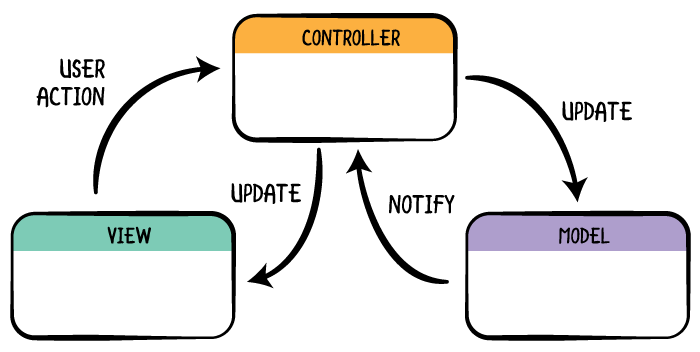
\includegraphics[width=0.5\linewidth]{img/mvc}
	\caption{Zusammenspiel des \ac{mvc}-Musters}
\end{figure}

% Erklärung MVC-Grafik

Technisch wird dieses Muster durch die Verknüpfung der einzelnen (durch den Interface Builder bereitgestellten oder erstellten) Views mit spezifischen, sog. \textit{View Controllern} realisiert. Durch eine Aktion des Nutzers auf dem View wird die entsprechende Funktionalität über den View Controller bereitgestellt. Dieser kann dann ebenfalls Funktionen ausführen, welche durch das Modell bereitgestellt werden, falls die Aktion dies bedarf. Die entsprechenden Klassen der View Controller sind Unterklassen der einzelnen, spezifischen Views, welche deren vorgesetzte Basisfunktionalitäten um die gewünschten Funktionen des Entwicklers erweitern.

\paragraph{Vorbereitung der Projektumgebung}\mbox{}\\
Bei der Erstellung eines neuen Projektes innerhalb von Xcode wählt der Entwickler bereits zu Beginn bestimmte Spezifikationen für die zu entwickelnde Anwendung. Da Swift auch für andere Betriebssysteme von Apple zur Anwendungsentwicklung genutzt wird, gehört die Spezifizierung des Anwendungsbereiches (hier: iOS) sowie des grundlegenden Aufbaus der App zu den Vorbereitungsmaßnahmen der Projektumgebung. Dieses Dialogfenster kann aus dem unten stehenden Screenshot entnommen werden.

\begin{figure}
	\centering
	\caption{Dialogfenster zum Anlegen eines neuen Projektes (Xcode)}
\end{figure}

Letztere bereiten verschiedene Dateitypen innerhalb der Umgebung vor, bspw. verschiedene Ansichten mit bereits integrierter Navigation, welche bei einer Anwendung mit nur einer Ansicht nicht zu tragen kommen. Im zweiten Schritt der Projektvorbereitung trifft der Entwickler Entscheidungen über Projektverzeichnis, -namen und -sprache sowie über weitere Projektkomponenten, welche für die Anwendung von Bedarf wären.

Alle hier getroffen Schritte können auch manuell bzw. im Nachgang der Projekterstellung angelegt werden. Grundsätzlich sind die Dateien und Quellcodezeilen, welche durch die genannten Vorbereitungsmaßnahmen automatisch generiert werden, unabdingbar für die Realisierung des Projekt und können somit für eine effizientere Arbeit des Entwicklers sorgen.

\paragraph{Struktur des initialen Entwicklungsverzeichnisses}
Bereits zu Anfang befinden sich bestimmte Dateien im Entwicklungsverzeichnis, welche sich grundsätzlich in jeder iOS-Anwendung benötigt werden. Diese werden im Folgenden beschrieben.

\begin{description}
	\item[\texttt{AppDelegate.swift}] ist der Eintrittspunkt der App. Dieser ist zuständig für das Verhalten der App, wenn diese (zum ersten Mal) geöffnet, geschlossen oder in den Hintergrund gerückt (d.\ h. inaktiv gesetzt) wird. Diese Datei ist vor allem dann von Interesse, wenn die Anwendung auch außerhalb ihrer Aktivität bestimmte Funktionen ausführt, bspw. also bei Musik-Anwendungen oder Stoppuhren. Aufgrund der automatischen Bereitstellung von Core Data zu Anfang des Projektes ist hier auch das Grundgerüst des \textit{Persistent Service} zu finden.
	\item[\texttt{SceneDelegate.swift}] ähnelt dem \texttt{AppDelegate} sehr, bezieht sich jedoch auf das Verhalten der Ansicht(-en) der Anwendung. Diese wird benötigt, da seit iOS-Version 13 auch mehrere offene Instanzen derselben App möglich sind, welche jedoch immer den aktuellsten Zustand darstellen sollen, unabhängig von der gerade aktiv laufenden Instanz. In Form einer Analogie aus der Web-Entwicklung kann man den \texttt{SceneDelegate} als die oberste Hierarchie der \textit{Frontend}-Steuerung bezeichnen, während das \textit{Back End} über den \texttt{AppDelegate} orchestriert wird.
	\item[\texttt{ViewController.swift}] ist einer von beliebig vielen möglichen Controllern, welche direkte Anbindung zu einer oder mehreren Ansichten hat. Dieser beinhaltet Konfigurationen der verschiedenen Komponenten der Ansicht und spezifiziert auch das Verhalten der Ansicht, wenn auf diese oder von dieser gewechselt wird.
	\item[\texttt{Main.storyboard}] ist das Gegenstück zu den \texttt{ViewController}. In Form eines sog. \textit{Interface Builders} können verschiedene Ansichten und deren Verknüpfungen via \textit{Drag-and-Drop} erstellt werden. Jede Ansicht wird mit genau einem \texttt{ViewController} versehen, welcher die Steuerung der definierten Elemente übernimmt. Grundsätzlich ist es auch möglich, vollständig ohne Interface Builder auszukommen. Die initiale Konfiguration der Positionen und der weiteren optischen Eigenschaften wird dann ebenfalls über den entsprechenden \texttt{ViewController} gehandhabt, wobei dies einen deutlich höheren Programmieraufwand aufweisen könnte. Neben des \texttt{Main.storyboard} existiert auch ein \texttt{LaunchScreen.storyboard}, welcher beim Laden der Anwendung ausgeführt wird.
	\item[\texttt{Assets.xcassets}] beinhaltet das App-Logo, welches im Menü des Mobilgerätes angezeigt wird. Dieses muss in fest definierten Größen bereitgestellt werden, wird jedoch an dieser Stelle vernachlässigt. Darüber hinaus können hier auch alle weiteren Grafiken, etc., abgelegt werden, welche innerhalb der App genutzt werden, um für eine ordnungsgemäße Skalierung der Symbole je nach Bildschirmgröße des Endgeräts zu gewährleisten.
	\item[\texttt{Info.plist}] ist eine allgemeine Konfigurationsdatei. Diese wird u.a. für Berechtigungen genutzt, welche die Anwendung außerhalb ihres eigenen Handlungsspielraums haben soll, bspw. die Nutzung der eingebauten Kameras, des GPS-Standortes des Geräts, die Berechtigung, Benachrichtigungen anzuzeigen, etc.
	\item[\texttt{to\_do.xcdatamodeld}] stellt die Konfigurationsdatei des Persistent Service dar, sofern dieser im Dialogfenster aktiviert wurde. In dieser werden Entitäten angelegt, mit möglichen Relationen versehen und für die Verwendung innerhalb der App exportiert.
\end{description}

\subsubsection{Vertrieb von iOS-Applikationen}
Der mit iOS 2.0 (Nachfolger von iPhone OS) ins Leben gerufene Apple \textit{App Store} ist die einzige offizielle Bezugsstelle für iOS-Applikationen. Somit ist es auch der am meisten verwendete Marktplatz, in welchem Entwickler und Unternehmen ihre Anwendung kostenlos sowie kostenpflichtig zum Download anbieten.

Zunächst ist die Anmeldung des Entwicklers als \textit{Apple Developer} im Vorhinein erforderlich. Ohne diese könnte die Anwendung zwar programmiert und innerhalb der Entwicklungsumgebung getestet, jedoch nicht auf tatsächlichen iOS-Geräten getestet und zum Download freigegeben werden. Dies hat sowohl sicherheitstechnische als auch wirtschaftliche Gründe, welche hier nicht weiter diskutiert, jedoch für die Evaluation der Entwicklungsfreiheit in Betracht gezogen werden. Letzteres erkennt man vor allem an der Tatsache, dass die Verbreitung von Anwendungen über den \textit{App Store} kostenpflichtig ist.

% Evtl. Quelle für die App-Publikation (iOS) finden und zitieren
Der genaue Prozess der Publikation von iOS-Applikationen kann im Rahmen dieser Arbeit nicht nachvollzogen werden, da keine Möglichkeit der tatsächlichen Bereitstellung der zu entwickelnden Beispielanwendung vorliegt.

\subsubsection{Nutzung von iOS-Applikationen}
Wie im vorigen Abschnitt erwähnt werden iOS-Anwendungen über den App Store bezogen. Auf weitere, inoffizielle und teils nonkonforme Praktiken wie das sog. \textit{Jailbraking} des Gerätes, um auch nicht-authorisierte Anwendungen herunterladen und nutzen zu können, wird hier nicht eingegangen.

Der iOS-Nutzer sucht über den App Store die gewünschte App und lädt diese herunter. Für diesen Prozess ist eine sog. \textit{Apple ID}, also ein Benutzerkonto bei Apple vonnöten. Sollte die gewünschte App kostenpflichtig sein, so müssen Kreditkarten- oder anderweitige, valide Zahlungsdaten dem Konto hinterlegt sein. Der Nutzer bestätigt den Kauf bzw. erstmaligen Download über das Benutzerkontenpasswort oder eine gerätespezifische Authentifizierungsmethode (bspw. Fingerabdruck-Erkennung via \textit{Touch ID} oder Gesichtserkennung via \textit{Face ID}, sofern vorhanden). Daraufhin startet der Download. Die App kann über ihr korrespondierendes App-Symbol, welches nun auf dem Menü-Bildschirm des Geräts erscheint, geöffnet werden.

Falls die App in einer nun aktuelleren Version vorliegt, wird diese entweder über den App Store automatisch im Hintergrund neu heruntergeladen. Andernfalls kann der Nutzer diesen Schritt auch manuell über den App Store in Kraft setzen.



\subsection{Android}

\textbf{Entwicklung}

%Android apps are written in Java and use various Java application program interfaces (APIs).
%Because you’ll want to write your own apps, but may be unfamiliar with the Java language and these
%APIs, this book teaches you about Java as a first step into Android app development. It provides you
%with Java language fundamentals and Java APIs that are useful when developing apps.

Native Android Anwendungen werden in Java entwickelt. Durch die Nutzung der zahlreichen APIs wird aus einem Java Programm eine native Android App.
\cite[S. 1]{JavaForAndroid}
Mittlerweile wird die teilweise veraltete Java-Syntax graduell durch die modernere Programmiersprache Kotlin abgelöst.
\cite{KotlinAndroid}


%Kotlin is a free and open source project under the Apache 2.0 license
%https://developer.android.com/kotlin

%https://kotlinlang.org/docs/reference/android-overview.html

Meist werden Android Apps mithilfe der Entwicklungsumgebung Android Studio entwickelt, welches auf der IntelliJ IDE von JetBrains aufbaut, aber von Google weiterentwickelt wird. Die IDE bietet Entwicklern unter anderem einen visuellen Layout-Editor und eine Vielzahl von Android Emulatoren zum Testen der Apps auf verschiedenen Android Versionen und unterschiedlicher Hardware. Dafür wird jedoch performante Hardware zum Entwickeln benötigt: 8 Gigabyte Arbeitsspeicher oder mehr ist die Empfehlung der Herausgeber. \cite{AndroidStudio}

\textbf{Vertrieb}

Die meisten Apps beziehen Nutzer über den Google Play Store, einem Onlineshop für kostenlose und kostenpflichtige Android Anwendungen. 
Updates werden ebenfalls über den Play Store installiert. Alternativ kann ein Nutzer eine App in Form einer \texttt{.apk}-Datei installieren. Dieser Weg bleibt jedoch aufgrund der Umständlichkeit und bedenklicher Sicherheit der App weitestgehend ungenutzt.




\subsection{Android}

\textbf{Entwicklung}

%Android apps are written in Java and use various Java application program interfaces (APIs).
%Because you’ll want to write your own apps, but may be unfamiliar with the Java language and these
%APIs, this book teaches you about Java as a first step into Android app development. It provides you
%with Java language fundamentals and Java APIs that are useful when developing apps.

Native Android Anwendungen werden in der Regel in Java entwickelt. Durch die Nutzung der zahlreichen APIs wird aus einem Java Programm eine native Android App.
\cite[S. 1]{JavaForAndroid}
Mittlerweile wird die teilweise veraltete Java-Syntax graduell durch die modernere Programmiersprache Kotlin abgelöst.
\cite{KotlinAndroid}


%Kotlin is a free and open source project under the Apache 2.0 license
%https://developer.android.com/kotlin

%https://kotlinlang.org/docs/reference/android-overview.html

Meist werden Android Apps mithilfe der Entwicklungsumgebung Android Studio entwickelt, welches auf der IntelliJ IDE von JetBrains aufbaut, aber von Google weiterentwickelt wird. Die IDE bietet Entwicklern unter anderem einen visuellen Layout Editor und eine Vielzahl von Android Emulatoren zum Testen der Apps auf verschiedenen Android Versionen und unterschiedlicher Hardware. Dafür wird jedoch performante Hardware zum Entwickeln benötigt: 8 Gigabyte Arbeitsspeicher oder mehr ist die Empfehlung der Herausgeber. \cite{AndroidStudio}

\textbf{Vertrieb}

Die meisten Apps beziehen Nutzer über den Google Play Store, einem Onlineshop für kostenlose und kostenpflichtige Android Anwendungen. 
Updates werden ebenfalls über den Play Store installiert. Alternativ kann ein Nutzer eine App in Form einer \texttt{.apk}-Datei installieren. Dieser Weg bleibt jedoch aufgrund der Umständlichkeit und unbekannten Sicherheitsprüfung der App weitestgehend ungenutzt.
